\documentclass[11pt]{article}
\usepackage{longtable}
\usepackage{graphicx}
\usepackage{lineno}
%\usepackage{amssymb}
\usepackage{color}
\definecolor{darkgreen}{rgb}{0,0.5,0}
\usepackage{hyperref}
\hypersetup{colorlinks=true, urlcolor=blue, citecolor=darkgreen}
\usepackage{natbib}
\usepackage{fullpage}
\usepackage{setspace}
\usepackage{listings}
\usepackage{scrextend}
\renewcommand{\familydefault}{\sfdefault}
\def\changemargin#1#2{\list{}{\rightmargin#2\leftmargin#1}\item[]}
\let\endchangemargin=\endlist 
\begin{document}
\begin{flushleft}


{\Large
\textbf{Improving transcriptome assembly through error correction of high-throughput sequence reads}
}
\\ 
\vspace{4mm}

\noindent
Matthew D MacManes$^{1}$$^\ast$ and
Michael B. Eisen$^{1,2}$ \\
\vspace{5mm}

\bf{1} \textnormal{UC Berkeley. California Institute of Quantitative Biology, Berkeley, CA, USA} \\
\bf{2} \textnormal{Howard Hughes Medical Institute} \\
\vspace{2mm}
 
\bf{$\ast$} \textnormal{Corresponding author: \href{mailto:macmanes@gmail.com}{macmanes@gmail.com}, Twitter: \href{https://twitter.com/PeroMHC}{$@$PeroMHC}}
\end{flushleft}
\vspace{4mm}

\section*{Supplementary Material}


\textbf{\hypertarget{Supplementary Figure 1}{Supplementary Figure 1}} \\
\centerline{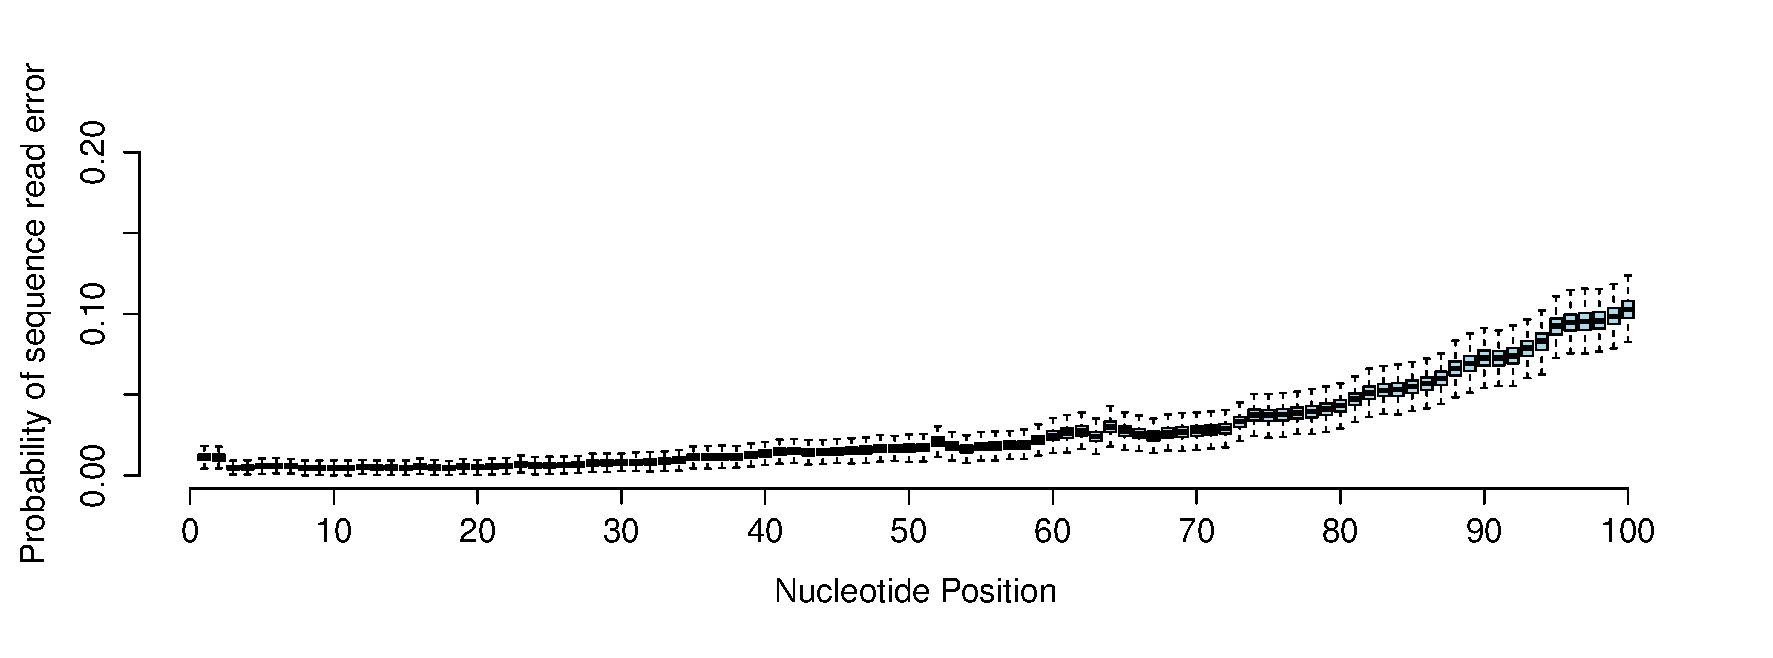
\includegraphics[width=30.0\baselineskip]{newfig1.eps}}
\noindent
\begin{changemargin}{2cm}{2cm} 
Figure1. The probability of error increases from the 5' to 3' end of the simulated sequencing reads. This error pattern is typical of Illumina sequencing.  
\end{changemargin}


\vspace{50mm}
\textbf{\hypertarget{Supplementary Figure 2}{Supplementary  Figure 2}} \\
\centerline{\includegraphics[width=30.0\baselineskip]{newfig2.eps}}
\begin{changemargin}{2cm}{2cm} 
Figure 2.  The log transformed distribution of gene expression (FPKM) in the simulated dataset. This pattern is typical of many well characterized Eukaryotic tissue types, where the vast majority of genes are expressed moderately, with much fewer being expressed at a very high level. 
\end{changemargin}
\vspace{10mm}


\end{document}